\documentclass[12pt]{report}
\usepackage[utf8]{inputenc}
\usepackage[english, russian]{babel}
\usepackage{listings}
\usepackage{graphicx}
\usepackage{float}
\graphicspath{{imgs/}}
\usepackage{amsmath,amsfonts,amssymb,amsthm,mathtools} 
\usepackage{pgfplots}
\usepackage{filecontents}
\usepackage{indentfirst}
\usepackage{eucal}
\usepackage{enumitem}
\frenchspacing

\usepackage{indentfirst} % Красная строка

\usetikzlibrary{datavisualization}
\usetikzlibrary{datavisualization.formats.functions}

\usepackage{amsmath}
\usepackage{fixltx2e}
\usepackage{caption}


\definecolor{bluekeywords}{rgb}{0,0,1}
\definecolor{greencomments}{rgb}{0,0.5,0}
\definecolor{redstrings}{rgb}{0.64,0.08,0.08}
\definecolor{xmlcomments}{rgb}{0.5,0.5,0.5}
\definecolor{types}{rgb}{0.17,0.57,0.68}

\usepackage{listings}
\lstset{language=[Sharp]C,
	captionpos=t,
	numbers=left, %Nummerierung
	numberstyle=\small, % kleine Zeilennummern
	frame=single, % Oberhalb und unterhalb des Listings ist eine Linie
	stepnumber=1,                   
	numbersep=5pt,                
	showspaces=false,
	tabsize=2,
	showtabs=false,
	breaklines=true,
	showstringspaces=false,
	breakatwhitespace=true,
	escapeinside={(*@}{@*)},
	commentstyle=\color{greencomments},
	morekeywords={partial, var, value, get, set},
	keywordstyle=\color{bluekeywords},
	stringstyle=\color{redstrings},
	basicstyle=\ttfamily\small,
}

\usepackage[left=2cm,right=2cm, top=2cm,bottom=2cm,bindingoffset=0cm]{geometry}
% Для измененных титулов глав:
\usepackage{titlesec, blindtext, color} % подключаем нужные пакеты
\definecolor{gray75}{gray}{0.75} % определяем цвет
\newcommand{\hsp}{\hspace{20pt}} % длина линии в 20pt
% titleformat определяет стиль
\titleformat{\chapter}[hang]{\Huge\bfseries}{\thechapter\hsp\textcolor{gray75}{|}\hsp}{0pt}{\Huge\bfseries}

\usepackage{array}
\newcommand{\head}[2]{\multicolumn{1}{>{\centering\arraybackslash}p{#1}}{#2}}

% plot
\usepackage{pgfplots}
\usepackage{filecontents}
\usetikzlibrary{datavisualization}
\usetikzlibrary{datavisualization.formats.functions}

\begin{document}
%\def\chaptername{} % убирает "Глава"
\thispagestyle{empty}
\begin{titlepage}
	\noindent \begin{minipage}{0.15\textwidth}
		
\includegraphics[width=\linewidth]{b_logo}
	\end{minipage}
	\noindent\begin{minipage}{0.9\textwidth}\centering
		\textbf{Министерство науки и высшего образования Российской Федерации}\\
		\textbf{Федеральное государственное бюджетное образовательное учреждение высшего образования}\\
		\textbf{~~~«Московский государственный технический университет имени Н.Э.~Баумана}\\
		\textbf{(национальный исследовательский университет)»}\\
		\textbf{(МГТУ им. Н.Э.~Баумана)}
	\end{minipage}
	
	\noindent\rule{18cm}{3pt}
	\newline\newline
	\noindent ФАКУЛЬТЕТ $\underline{\text{«Информатика и системы управления»}}$ \newline\newline
	\noindent КАФЕДРА $\underline{\text{«Программное обеспечение ЭВМ и информационные технологии»}}$\newline\newline\newline\newline\newline\newline\newline\newline\newline\newline\newline
	
	
	\begin{center}
		\noindent\begin{minipage}{1.3\textwidth}\centering
			\Large\textbf{  Отчет по лабораторной работе №6}\newline
			\textbf{по дисциплине "Анализ алгоритмов"}\newline\newline
		\end{minipage}
	\end{center}
	
	\noindent\textbf{Тема} $\underline{\text{Муравьиный алгоритм и метод полного перебора для решения задачи коммивояжёра}}$\newline\newline
	\noindent\textbf{Студент} $\underline{\text{Малышев И. А.}}$\newline\newline
	\noindent\textbf{Группа} $\underline{\text{ИУ7-51Б}}$\newline\newline
	\noindent\textbf{Оценка (баллы)} $\underline{\text{~~~~~~~~~~~~~~~~~~~~~~~~~~~}}$\newline\newline
	\noindent\textbf{Преподаватель: } $\underline{\text{Волкова Л. Л.}}$\newline\newline\newline
	
	\begin{center}
		\vfill
		Москва~---~\the\year
		~г.
	\end{center}
\end{titlepage}


\renewcommand{\contentsname}{Содержание}
\tableofcontents
\setcounter{page}{2}

\newpage
\chapter*{Введение}
\addcontentsline{toc}{chapter}{Введение}
Коммивояжёр (фр. commis voyageur) — бродячий торговец. Задача коммивояжёра — важная задача транспортной логистики, отрасли, занимающейся планированием транспортных перевозок. Коммивояжёру, чтобы распродать нужные и не очень нужные в хозяйстве товары, следует объехать n пунктов и в конце концов вернуться в исходный пункт. Требуется определить наиболее выгодный маршрут объезда. В качестве меры выгодности маршрута (точнее говоря, невыгодности) может служить суммарное время в пути, суммарная стоимость дороги, или, в простейшем случае, длина маршрута \cite{commi1}.

        
\textbf{Целью} данной лабораторной работы является изучение муравьиных алгоритмов и приобретение навыков параметризации методов на примере муравьиного алгоритма, примененного к задаче коммивояжера.
        
\textbf{Задачи} данной лабораторной работы:
\begin{itemize}
	\item рассмотренть муравьиный алгоритм и алгоритм полного перебора для решения задачи коммивояжера;
	\item реализовать эти алгоритмы;
	\item провести параметризацию муравьиного алгоритма;
	\item сравнить время работы этих алгоритмов.
\end{itemize}



\chapter{Аналитическая часть}
В данной части будут рассмотрены теоретические основы задачи коммивояжера и рассматриваемых алгоритмов для её решения. 
		
\section{Постановка задачи} 
Имеется сильно связный взвешенный ориентированный граф \cite{diskr} с положительными весами, заданный в виде матрицы смежностей. Количество вершин в нем лежит в диапазоне от 5 до 20. Требуется решить задачу коммивояжера для этого графа. 

\section{Решение полным перебором}
Задача может быть решена перебором всех вариантов объезда и выбором оптимального. Но при таком подходе количество возможных маршрутов очень быстро возрастает с ростом n (количество маршрутов равно $n!$ — количеству способов упорядочивания пунктов). Уже при относительно небольшом числе городов (66 и более) она не может быть решена методом перебора вариантов никакими теоретически мыслимыми компьютерами за время, меньшее нескольких миллиардов лет. 

Не спасает ситуацию даже то, что для каждого варианта маршрута имеется $2n$ равноценных, отличающихся выбором начального пункта ($n$ вариантов) и направлением обхода (2 варианта). Перебор с учётом этого наблюдения сокращается незначительно \cite{commi2}.	

\section{Муравьиные алгоритмы}
Все муравьиные алгоритмы базируются на моделировании поведения колонии муравьев. Колония муравьев может рассматриваться как многоагентная система, в которой каждый агент (муравей) функционирует автономно по очень простым правилам. В противовес почти примитивному поведению агентов, поведение всей системы получается на удивление разумным.
		
Муравьиные алгоритмы представляют собой вероятностную жадную эвристику, где вероятности устанавливаются, исходя из информации о качестве решения, полученной из предыдущих решений.

Идея муравьиного алгоритма - моделирование поведения муравьёв, связанного с их способностью быстро находить кратчайший путь от муравейника к источнику пищи и адаптироваться к изменяющимся условиям, находя новый кратчайший путь \cite{shtovba}. При своём движении муравей метит путь феромоном, и эта информация используется другими муравьями для выбора пути. Это элементарное правило поведения и определяет способность муравьёв находить новый путь, если старый оказывается недоступным.

Какие же механизмы обеспечивают столь сложное поведение муравьев, и что можем мы позаимствовать у этих крошечных существ для решения своих глобальных задач? Основу «социального» поведения муравьев составляет самоорганизация — множество динамических механизмов, обеспечивающих достижение системой глобальной цели в результате низкоуровневого взаимодействия ее элементов. Принципиальной особенностью такого взаимодействия является использование элементами системы только локальной информации. При этом исключается любое централизованное управление и обращениек глобальному образу, репрезентирующему систему во внешнем мире. Самоорганизация является результатом взаимодействия следующих четырех компонентов \cite{shtovba} :

\begin{itemize}
	\item случайность;
	\item многократность;
	\item положительная обратная связь;
	\item отрицательная обратная связь.
\end{itemize}

Рассмотрим случай, когда на оптимальном на данный момент пути возникает преграда. В этом случае необходимо определение нового оптимального пути. Дойдя до преграды, муравьи с равной вероятностью будут обходить её справа и слева. То же самое будет происходить и на обратной стороне преграды. Однако, те муравьи, которые случайно выберут кратчайший путь, будут быстрее его проходить, и за несколько передвижений он будет более обогащён феромоном. Поскольку движение муравьёв определяется концентрацией феромона, то следующие будут предпочитать именно этот путь, продолжая обогащать его феромоном до тех пор, пока этот путь по какой-либо причине не станет недоступен.

Очевидная положительная обратная связь быстро приведёт к тому, что кратчайший путь станет единственным маршрутом движения большинства муравьёв. Моделирование испарения феромона - отрицательной обратной связи - гарантирует нам, что найденное локально оптимальное решение не будет единственным - муравьи будут искать и другие пути. Если мы моделируем процесс такого поведения на некотором графе, рёбра которого представляют собой возможные пути перемещения муравьёв, в течение определённого времени, то наиболее обогащённый феромоном путь по рёбрам этого графа и будет являться решением задачи, полученным с помощью муравьиного алгоритма.

Обобщим все выше сказанное. Любой муравьиный алгоритм, независимо от модификаций, представим в следующем виде:
\begin{itemize}
	\item создание муравьев;
	\item поиск решения;
	\item обновление феромона;
	\item дополнительные действия (опиционально).
\end{itemize}

Сложность алгоритма: $O(t_{max} * max(m, n^2))$, где $t_{max}$ --- время жизни колонии, $m$ --- количество муравьев в колонии, $n$ --- размер графа \cite{shtovba}.

Теперь рассмотрим каждый шаг в цикле более подробно.

\subsection{Создание муравьев}

Стартовая точка, куда помещается муравей, зависит ограничений,   накладываемых условиями задачи. Потому что для каждой задачи   способ размещения муравьёв является определяющим. Либо все    они помещаются в одну точку, либо в разные с повторениями, либо без повторений.

На этом же этапе задается начальный уровень феромона. Он    инициализируется небольшим положительным числом для того,    чтобы на начальном шаге вероятности перехода в следующую    вершину не были нулевыми. 
  
\subsection{Поиск решения}

 Вероятность перехода из вершины i в вершину j определяется по следующей формуле\ref{form:way}\\   
\begin{equation}\label{form:way} 
 p_{i,j}={\frac {(\tau _{i,j}^{\alpha })(\eta _{i,j}^{\beta })}{\sum (\tau _{i,j}^{\alpha })(\eta _{i,j}^{\beta })}}
 \end{equation}
    где \quad$ \tau _{i,j} - $ расстояние от города $i$ до города $j$;
    
         $\eta _{i,j} - $количество феромонов на ребре $ij$;
         
          $\alpha - $ параметр влияния длины пути;
          
          $\beta - $ параметр влияния феромона.


\subsection{Обновление феромона}

  Уровень феромона обновляется в соответствии с приведённой формулой:\\
После того, как муравей успешно проходит маршрут, он оставляет на всех пройденных ребрах след, обратно пропорциональный длине пройденного пути. Итого, новый след феромона вычисляется по формуле \ref{form:eva}:
\begin{equation}\label{form:eva} 
    \eta _{i,j}=(1-\rho )\eta _{i,j}+\Delta \eta _{i,j},
\end{equation}
где \quad$ \rho _{i,j}$ - \text{доля феромона, который испарится;} 

    $\eta _{i,j}$ - \text{количество феромона на дуге ij;} 
    
    $\Delta \eta _{i,j}$ - \text{количество отложенного феромона, вычисляется по формуле \ref{form:add1}.}


\section{Муравьиный алгоритм в задаче коммивояжера}
Рассмотрим, как реализовать четыре составляющие самоорганизации муравьев при оптимизации маршрута коммивояжера. Многократность взаимодействия реализуется итерационным поиском маршрута коммивояжера одновременно несколькими муравьями. При этом каждый муравей рассматривается как отдельный, независимыйкоммивояжер, решающий свою задачу. За однуитерацию алгоритма каждый муравей совершаетполный маршрут коммивояжера.Положительная обратная связь реализуется как имитация поведения муравьев типа «оставление следов – перемещение по следам». Чем больше следов оставлено на тропе — ребре графа в задаче коммивояжера, тем больше муравьев будет передвигаться по ней. При этом на тропе появляются новые следы, привлекающие дополнительных муравьев. Для задачи коммивояжера положительная обратная связь реализуется следующим стохастическим правилом: вероятность включения ребра графа в маршрут муравья пропорциональна количеству феромона на нем.
		
Теперь с учетом особенностей задачи коммивояжёра, мы можем описать локальные правила поведения муравьев при выборе пути:

\begin{enumerate}	
	\item Муравьи имеют собственную «память». Поскольку каждый город может быть посещён только один раз, то у каждого муравья есть список уже посещенных городов - список запретов. Обозначим через $J$ список городов, которые необходимо посетить муравью $k$ , находящемуся в городе $i$. 
	
	\item Муравьи обладают «зрением» - видимость есть эвристическое желание посетить город $j$ , если муравей находится в городе $i$ . Будем считать, что видимость обратно пропорциональна расстоянию между городами. 
	
	\item Муравьи обладают «обонянием» - они могут улавливать след феромона, подтверждающий желание посетить город $j$ из города $i$ на основании опыта других муравьёв. Количество феромона на ребре $(i,j)$ в момент времени $t$ обозначим через  $\eta _{i,j} (t)$ 
	
	\item На этом основании мы можем сформулировать вероятностнопропорциональное правило, определяющее вероятность перехода $k$-ого муравья из города $i$  в город $j$. 
	 
	\item Пройдя ребро $(i,j)$ , муравей откладывает на нём некоторое количество феромона, которое должно быть связано с оптимальностью сделанного выбора. Пусть $T _{k} (t)$ есть маршрут, пройденный муравьем $k$ к моменту времени $t$ , $L _{k} (t)$ - длина этого маршрута, а $Q$ - параметр, имеющий значение порядка длины оптимального пути. Тогда откладываемое количество феромона может быть задано в виде:
	  \begin{equation}\label{form:add} 
	 	{\displaystyle \Delta \eta _{i,j}^k={\begin{cases}Q/L_{k}& {\mbox{Если $k$-ый мурваей прошел по ребру $ij$;}}\\0&{\mbox{Иначе}}\end{cases}}}
	 \end{equation}
	 где $Q$ - количество феромона, переносимого муравьем;
	 
	 тогда
	 \begin{equation}\label{form:add1} 
	 	\Delta \eta _{i,j}= \eta _{i,j}^0 + \eta _{i,j}^1 + ... + \eta _{i,j}^k 
	 \end{equation}
	 
	 где k - количество муравьев в вершине графа с индексами i и j.
\end{enumerate}


\section*{Вывод}
\addcontentsline{toc}{section}{Вывод}
В данном разделе были рассмотрены общие принципы муравьиного алгоритма и применение его к задаче коммивояжера. 


\newpage
\chapter{Конструкторская часть}
В данном разделе будут рассмотрены основные требования к программе и схемы алгоритмов.

\section{Требования к программе}
\noindent Требования к вводу:
\begin{itemize}
	\item у неориентированного графа должно быть хотя бы 2 вершины.
\end{itemize}

""\newline
Требования к программе:
\begin{itemize}
	\item алгоритм полного перебора должен возвращать кратчайший путь в графе.
\end{itemize}
 .  
\newline  
Входные данные: матрица смежности графа.  
\newline
Выходные данные: самый выгодный путь.

\section{Схемы алгоритмов}
На рисунках 2.1 и 2.2 приведены схемы алгоритмов решения задачи коммивояжера.

\begin{figure}[H]
        	\centering
        	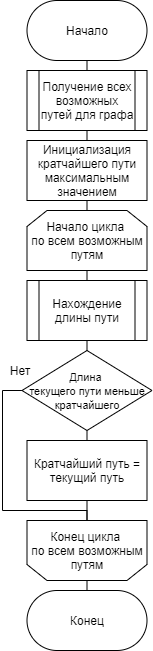
\includegraphics[scale = 0.8]{BruteForce.png}
        	\caption{Схема алгоритма полного перебора}
        	\label{fig:f_p}
\end{figure}  

\begin{figure}[H]
        	\centering
        	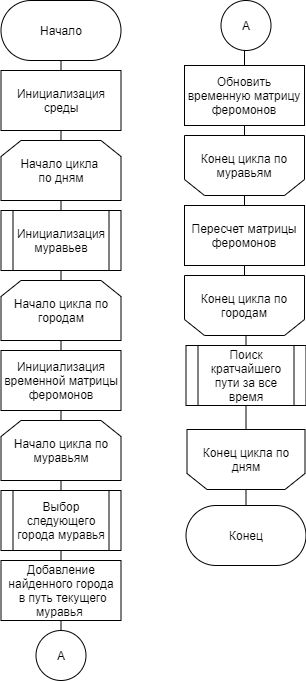
\includegraphics[scale = 0.8]{Ant.png}
        	\caption{Схема муравьиного агоритма}
        	\label{fig:ant}
\end{figure}


\section*{Вывод}
\addcontentsline{toc}{section}{Вывод}
В данном разделе были рассмотрены требования к программе и схемы алгоритмов.
 
\newpage
\chapter{Технологическая часть}
Замеры времени были произведены на процессоре Intel(R) Core(TM) i7-4790K, 4 ядра, 8 логических процессоров.

\section{Средства реализации}
В качестве языка программирования был выбран C\# \cite{Microsoft}, а среды разработки -- Visual Studio, т. к. я знаком с данным языком и имею представление о тестировании программ в данном языке. Время работы алгоритмов было замерено с помощью библиотеки System.Diagnostics, класса Stopwatch, который имеет методы для расчёта процессорного времени.


\section{Реализация алгоритмов}
В этой части будут рассмотрены листинги кода (листинг 3.1 - 3.3) реализованых алгоритмов.

\captionsetup{singlelinecheck = false, justification=raggedright}
\begin{lstlisting}[label=some-code,caption=Алгоритм поиска полным перебором]
public static Path GetShortestPath(Map m)
{
    int[] routeIndexes = new int[m.n - 1];
    for (int i = 0; i < m.n - 1; i++)
    {
        routeIndexes[i] = i + 1;
    }
    var allRoutes = GetAllRoutes(routeIndexes);
    Path shortestPath = new Path(int.MaxValue);
    foreach (List<int> path in allRoutes)
    {
        path.Insert(0, 0);
        path.Add(0);
        Path cur = new Path(m, path.ToArray());
        if (cur.distance < shortestPath.distance)
            shortestPath = cur;
    }

    return shortestPath;
}
\end{lstlisting}

\begin{lstlisting}[label=some-code,caption=Алгоритм поиска всех перестановок]
public static List<List<T>> GetAllRoutes<T>(IList<T> arr, List<List<T>> res = null, List<T> current = null)
{
    if (res == null)
        res = new List<List<T>>();
    if (arr.Count == 0)
    {
        res.Add(current);
        return res;
    }
    for (int i = 0; i < arr.Count; i++)
    {
        List<T> lst = new List<T>(arr);
        lst.RemoveAt(i);
        List<T> next;
        if (current == null)
            next = new List<T>();
        else
            next = new List<T>(current);
        next.Add(arr[i]);
        GetAllRoutes(lst, res, next);
    }
    return res;
}
\end{lstlisting}

\newpage

\begin{lstlisting}[label=some-code,caption=Муравьиный алгоритм]
public static Path GetShortestPath(Map map, int nIter, double alpha, double beta, double Q, double ro)
{
    Path minPath = new Path(int.MaxValue);
    int n = map.n;
    double[][] pheromones = Program.InitMatr(n, 0.1);

    List<Ant> ants;
    for (int t = 0; t < nIter; t++) // days
    {
        ants = InitAnts(map, n);

        // colony route
        for (int i = 0; i < n - 1; i++)
        {
            double[][] pheromonesIter = Program.InitMatr(n, (double)0); // 1 colony step

            for (int j = 0; j < ants.Count(); j++) // ants
            {
                double sumChance = 0, chance = 0;
                Ant curAnt = ants[j];
                int curCity = curAnt.path.route.Last();
                for (int cityId = 0; cityId < n; cityId++) 
                {
                    if (curAnt.visited[cityId] == false)
                    {
                        sumChance += Math.Pow(pheromones[curCity][cityId], alpha) * Math.Pow(1.0 / (map.distance[curCity][cityId]), beta);
                    }
                }
                double x = r.NextDouble();
                int k = 0;
                for (; x > 0; k++)
                {
                    if (curAnt.visited[k] == false)
                    {
                        chance = Math.Pow(pheromones[curCity][k], alpha) * Math.Pow(1.0 / (map.distance[curCity][k]), beta);
                        chance /= sumChance;
                        x -= chance;
                    }
                }
                k--;
                ants[j].VisitedTown(k);
                pheromonesIter[curCity][k] += Q / (map.distance[curCity][k]);
            }

            for (int ii = 0; ii < n; ii++)
                for (int j = 0; j < n; j++)
                    pheromones[ii][j] = (1 - ro) * pheromones[ii][j] + pheromonesIter[ii][j];
        }
        
        foreach (Ant a in ants)
        {
            a.VisitedTown(a.iStartTown);
            if (a.GetDistance() < minPath.distance)
            {
                minPath = a.path;
            }
        }                
    }
    return minPath;
}
\end{lstlisting}

\captionsetup{singlelinecheck = false, justification=centering}

\section*{Вывод}
\addcontentsline{toc}{section}{Вывод}
В данном разделе были рассмотрены основные сведения о модулях программы и листинг кода алгоритмов.

\newpage
\chapter{Исследовательская часть}
В даннном разделе будет проведен сравнительный временной анализ алгоритмов и рассмотрена параметризация муравьиного алгоритма.

\section{Сравнительный анализ на основе замеров времени}
Был проведен замер времени работы алгоритмов при разных размерах графа. На рис. 4.1 и рис. 4.2 показаны результаты замеров времени.

\begin{center}
\begin{tikzpicture}
\begin{axis}[
    	axis lines = left,
    	xlabel = {Количество вершин},
    	ylabel = {Время (тики)},
	legend pos=north west,
	ymajorgrids=true
]

\addplot[color=blue] table[x index=0, y index= 1] {Brute.txt}; 
\addlegendentry{Полный перебор}

\addplot[color=orange] table[x index=0, y index= 1] {Ant.txt}; 
\addlegendentry{Муравьиный алгоритм}

\end{axis}
\end{tikzpicture}
\end{center}

\begin{center}
Pис. 4.1. Сравнение времени работы алгоритмов при увеличении размера графа.
\end{center}

\begin{center}
\begin{tikzpicture}
\begin{axis}[
    	axis lines = left,
    	xlabel = {Количество вершин},
    	ylabel = {Время (тики)},
	legend pos=north west,
	ymajorgrids=true
]


\addplot[color=blue] table[x index=0, y index= 1] {Brute2.txt}; 
\addlegendentry{Полный перебор}

\addplot[color=orange] table[x index=0, y index= 1] {Ant2.txt}; 
\addlegendentry{Муравьиный алгоритм}


\end{axis}
\end{tikzpicture}
\end{center}

\begin{center}
Pис. 4.2. Сравнение времени работы алгоритмов на малых размерах графа.
\end{center}

На рисунках 4.1 и 4.2 видно, что муравьиный алгоритм значительно выигрывает по скорости полному перебору при размере графа больше 9.
До 8 вершин алгоритм полного перебора работает быстрее, с максимальным выигрышем по времени в 2,5 раза, при 6 вершинах.
На графе размера 10 полный перебор работает в 30 раз медленнее. 

\section{Параметризация муравьиного алгоритма}	

Пусть $t_{max} = 100$, $Q = 5$ и $n = 10$. Для различных значений параметров $\alpha$, $\beta$ и $\rho$ для каждой из нескольких матриц смежности с помощью муравьиного алгоритма и перебора была найдена некоторая длина маршрута. Длина маршрута, найденная перебором, считается эталонной. Далее выбраны наилучшие сочетания параметров муравьиного алгоритма на основе совпадения с эталоном.

Параметр $\alpha$ менялся от 0 до 1 с шагом 0.1, параметр $\rho$ менялся от 0 до 1 с шагом 0.1.

Итого были выявлены оптимальные сочетания параметров (представлены в таблице 4.1):

\begin{table}[H]
	\caption{Результаты решения задачи параметризации}
	\begin{center}
		
	\begin{tabular}{|c|c|c|}
		\hline
		$\alpha$ &$\beta = 1 - \alpha$ & $\rho$ \\\hline
		 
		0.1&0.9&0.3\\
		0.1&0.9&0.4\\
		0.1&0.9&0.6\\
		 
		0.2&0.8&0.1\\
		0.2&0.8&0.2\\
		0.2&0.8&0.3\\
		0.2&0.8&0.4\\
		 
		0.3&0.7&0.1\\
		0.3&0.7&0.2\\
		0.3&0.7&0.5\\
		 
		0.4&0.6&0.1\\
		0.4&0.6&0.2\\
		 
		0.5&0.5&0.1\\
		0.5&0.5&0.2\\
		\hline
	\end{tabular}
\end{center}
\end{table} 
\

\section*{Вывод}
\addcontentsline{toc}{section}{Вывод}
Сравнительный анализ по времени показал, что на больших размерностях (размер графа больше 9) полный перебор крайне медленен относительно муравьиного алгоритма.

Наиболее стабильные результаты автоматической параметризации получаются при наборе $\alpha = 0.1..0.5$, $\beta = 0.5..0.9$, $\rho = $ любое. При таких параметрах полученный результат в большинстве случаев (в около 75\%) полученный результат совпадает с эталонным. Наиболее нестабильные результаты полученны при $\alpha = 1.0$, $\beta = 0.0$, $\rho = $ любое.


\chapter*{Заключение}
\addcontentsline{toc}{chapter}{Заключение}
В рамках данной лабораторной работы лабораторной работы была достигнута её цель: изучен муравьиный алгоритм и приобретены навыки параметризации методов на примере муравьиного алгоритма. Также выполнены следующие задачи:

\begin{itemize}
	\item реализованны два алгоритма решения задачи коммивояжера;
	\item замерено время выполнения алгоритмов;
	\item муравьиный алгоритм протестирован на разных переменных;
	\item сделаны выводы на основе проделанной работы.
\end{itemize}

Поставленная цель была достигнута.

\newpage
\addcontentsline{toc}{chapter}{Список литературы}
\renewcommand\bibname{Список литературы}
 \begin{thebibliography}{3}
 	\bibitem{commi1} Т.М. Товстик, Е.В. Жукова - Алгоритм приближенного решения задачи коммивояжера.
 	\bibitem{diskr} Белоусов А.И., Ткачев С.Б(2006). Дискретная математика, 4-е издание.
 	http://mech.math.msu.su/~shvetz/54/inf/perl-problems/chCommisVoyageur.xhtml
 	\bibitem{commi2} Задача коммивояжера [Электронный ресурс] - режим доступа
 	\bibitem{shtovba} Штовба С.Д. - Муравьиные алгоритмы.
	\bibitem{Microsoft} Руководство по языку C\# [Электронный ресурс], - режим доступа: https://docs.microsoft.com/ru-ru/dotnet/csharp/
\end{thebibliography}


\end{document}